\section{Application-Layer Validation: Edge and Ground Processing}
\label{sec:testing-detection}

\subsection{Experimental Setup and Evaluation Procedure}
\label{subsec:testing-detection-setup}

The final comparison evaluated the Edge and Ground processing modes described in Chapter~3. The \ac{UAV} pose and camera view were kept unchanged, and both modes used the same detector settings. In Edge mode, detection was performed before results were delivered to the \ac{GCS}. In Ground mode, JPEG images were transferred through the \ac{NS-3} network path and processed at the \ac{GCS}. Table~\ref{tab:application-test-configuration} lists the controlled settings.

\begin{table}[H]
    \centering
    \caption{Configuration used for the application-layer validation.}
    \label{tab:application-test-configuration}
    \begin{tabular}{|l|l|}
        \hline
        Parameter & Value \\ \hline
        \ac{UAV} latitude & 6.079430 degrees \\ \hline
        \ac{UAV} longitude & 80.193085 degrees \\ \hline
        Relative altitude & 25.0 m \\ \hline
        Yaw & 102.6 degrees \\ \hline
        Camera relay rate & 1 Hz \\ \hline
        Official measurement duration & 60 s \\ \hline
        YOLO model & YOLOv8n \\ \hline
        Confidence threshold & 0.25 \\ \hline
        Target class & person \\ \hline
        Ground JPEG quality & 5 \\ \hline
        \ac{NS-3} RNG runs & 1, 2 and 3 \\ \hline
        Independent repetitions & 3 per mode \\ \hline
        Debug-image publication & disabled \\ \hline
        Minimum processed warm-up rows & 9 \\ \hline
        Post-warm-up settling period & 15 s \\ \hline
        Stability requirement & 5 consecutive stable arrivals \\ \hline
    \end{tabular}
\end{table}

The analysis used the metadata-defined official window for each run. Startup rows were excluded before the 15~s settling check, and measurement began only after five consecutive stable arrivals. One complete run was treated as one independent repetition; individual frames were not treated as separate experimental repetitions. The processed-frame ratio is the proportion of frames published by the camera relay during the official measurement window that produced a corresponding detection-result record within that window.

\subsection{Detection Accuracy under JPEG Compression}
\label{subsec:testing-detection-accuracy}

A separate labelled-frame test compared the detector output from raw images with output from the same images compressed at JPEG quality~5. Table~\ref{tab:d4-detection-accuracy} gives the verified results at the common confidence threshold of 0.25.

\begin{table}[H]
    \centering
    \caption{Detection accuracy for raw and JPEG-quality-5 images.}
    \label{tab:d4-detection-accuracy}
    \begin{tabular}{|l|c|c|c|c|}
        \hline
        Mode & Precision & Recall & F1-score & Exact-count rate \\ \hline
        Edge/raw & 0.878205 & 0.810651 & 0.843077 & 0.557377 \\ \hline
        Ground/JPEG q5 & 1.000000 & 0.171598 & 0.292929 & 0.426230 \\ \hline
    \end{tabular}
\end{table}

Ground/JPEG q5 produced no false-positive detections in this test, which gave a precision of 1.000000. However, its recall was only 0.171598, so this precision value does not mean that it was more accurate overall. The raw-image result retained much more of the labelled person detections and therefore had the higher F1-score.

\begin{figure}[H]
    \centering
    \IfFileExists{images/application_layer_validation/d4_detection_accuracy_comparison.pdf}{%
        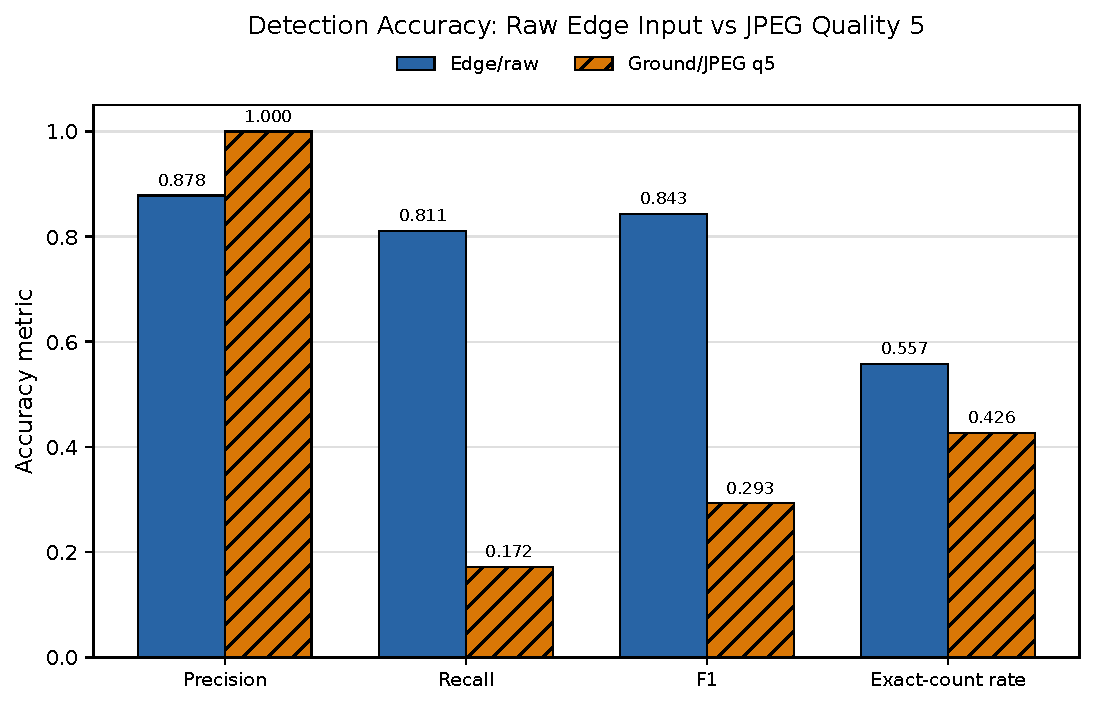
\includegraphics[width=0.78\textwidth]{images/application_layer_validation/d4_detection_accuracy_comparison.pdf}%
    }{%
        \fbox{\parbox[c][0.28\textheight][c]{0.85\textwidth}{\centering Figure file not found.}}%
    }
    \caption{Detection accuracy comparison between raw images and JPEG-quality-5 images.}
    \label{fig:d4-detection-accuracy-comparison}
\end{figure}

\subsection{Processed-Frame Reliability and Pipeline Latency}
\label{subsec:testing-detection-reliability-latency}

From this point, values written as mean $\pm$ sample standard deviation are calculated across three independent runs. The per-run processed-frame results are shown in Table~\ref{tab:processed-frame-results}. Every frame published during the official Edge measurement windows produced a corresponding detection-result record. Ground processing produced fewer result records than Edge processing, although the missing records may include several pipeline and communication effects and are not attributed only to radio packet loss.

\begin{table}[H]
    \centering
    \caption{Official processed-frame results for each RNG run.}
    \label{tab:processed-frame-results}
    \begin{tabular}{|c|c|c|c|c|}
        \hline
        & \multicolumn{2}{c|}{Edge} & \multicolumn{2}{c|}{Ground} \\ \hline
        RNG run & Processed/sent & Ratio & Processed/sent & Ratio \\ \hline
        1 & 58/58 & 1.0000 & 49/60 & 0.8167 \\ \hline
        2 & 60/60 & 1.0000 & 48/60 & 0.8000 \\ \hline
        3 & 60/60 & 1.0000 & 41/60 & 0.6833 \\ \hline
    \end{tabular}
\end{table}

The Edge processed-frame ratio was $1.0000 \pm 0.0000$, compared with $0.7667 \pm 0.0727$ for Ground. This is an Edge completion advantage of 23.33 percentage points under the tested configuration.

\begin{figure}[H]
    \centering
    \IfFileExists{images/application_layer_validation/processed_frame_ratio_by_rng.pdf}{%
        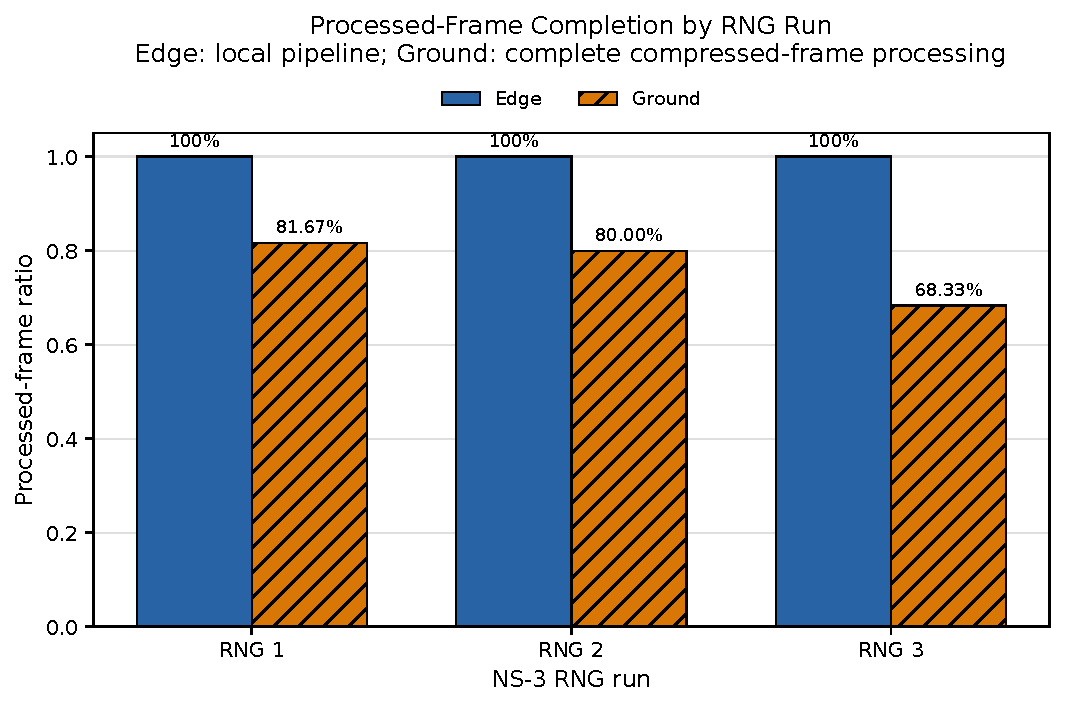
\includegraphics[width=0.78\textwidth]{images/application_layer_validation/processed_frame_ratio_by_rng.pdf}%
    }{%
        \fbox{\parbox[c][0.28\textheight][c]{0.85\textwidth}{\centering Figure file not found.}}%
    }
    \caption{Processed-frame ratio for Edge and Ground processing across the three RNG runs.}
    \label{fig:processed-frame-ratio-by-rng}
\end{figure}

The mean of the run-level median latencies was $182.41 \pm 19.22$~ms for Edge and $507.86 \pm 4.34$~ms for Ground. Ground was therefore 325.45~ms higher, or 2.78 times the Edge value. The mean of the three run-level p95 values was $421.25 \pm 170.22$~ms for Edge and $562.97 \pm 5.43$~ms for Ground. These are summaries of the run-level statistics, not pooled frame-level medians or confidence intervals.

\begin{figure}[H]
    \centering
    \IfFileExists{images/application_layer_validation/median_pipeline_latency_by_rng.pdf}{%
        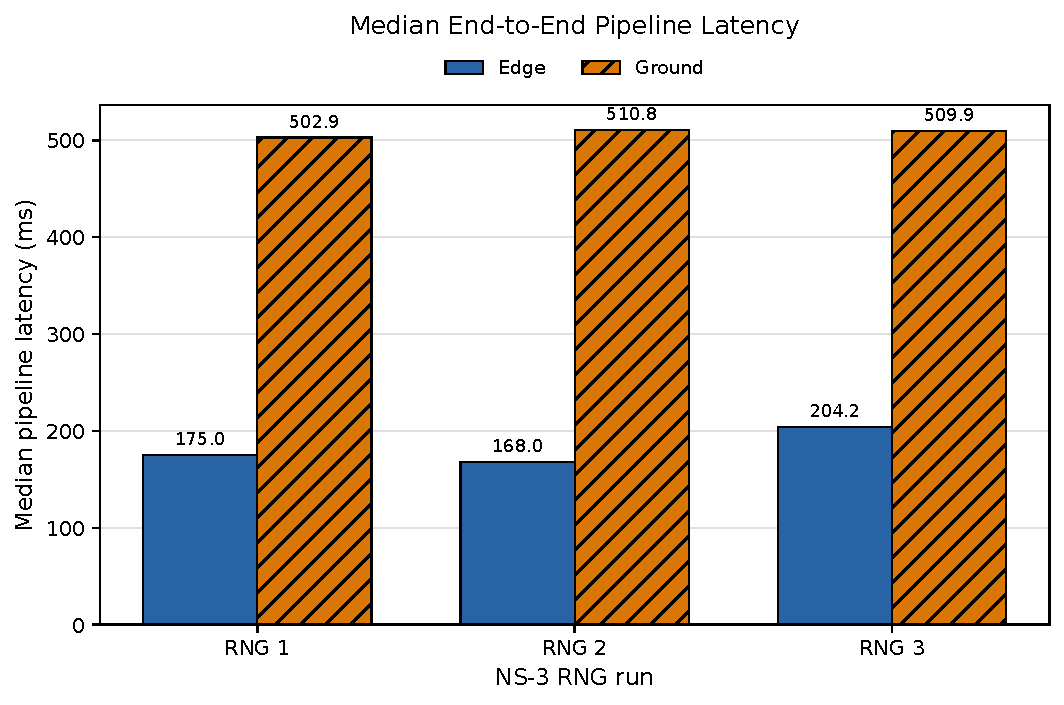
\includegraphics[width=0.78\textwidth]{images/application_layer_validation/median_pipeline_latency_by_rng.pdf}%
    }{%
        \fbox{\parbox[c][0.28\textheight][c]{0.85\textwidth}{\centering Figure file not found.}}%
    }
    \caption{Run-level median pipeline latency for Edge and Ground processing.}
    \label{fig:median-pipeline-latency-by-rng}
\end{figure}

\subsection{Inference and Resource Utilisation}
\label{subsec:testing-detection-resources}

Mean inference time was $54.52 \pm 3.12$~ms for Edge and $51.57 \pm 4.92$~ms for Ground, so the inference times were similar in both modes. For Ground processing, mean compression time was $2.51 \pm 0.05$~ms and mean decoding time was $2.14 \pm 0.15$~ms. Their combined mean was 4.64~ms. Compression and decoding alone therefore did not explain the full pipeline-latency difference. The remaining time may include communication, \ac{ROS} DDS processing, serialisation, queueing, scheduling, and other pipeline delays.

CPU and RSS were measured on the simulation host for the monitored detector-plus-relay process set. Mean monitored CPU was $56.22 \pm 2.56\%$ for Edge and $42.44 \pm 1.47\%$ for Ground. The monitored Edge-mode process set used more mean CPU than the monitored Ground-mode process set. Mean monitored RSS was $952.32 \pm 5.11$~MB for Edge and $963.34 \pm 2.58$~MB for Ground, which indicates similar memory use in the two modes. These host measurements do not represent physical \ac{UAV} energy or total platform power.

\begin{figure}[H]
    \centering
    \IfFileExists{images/application_layer_validation/mean_cpu_utilization_by_rng.pdf}{%
        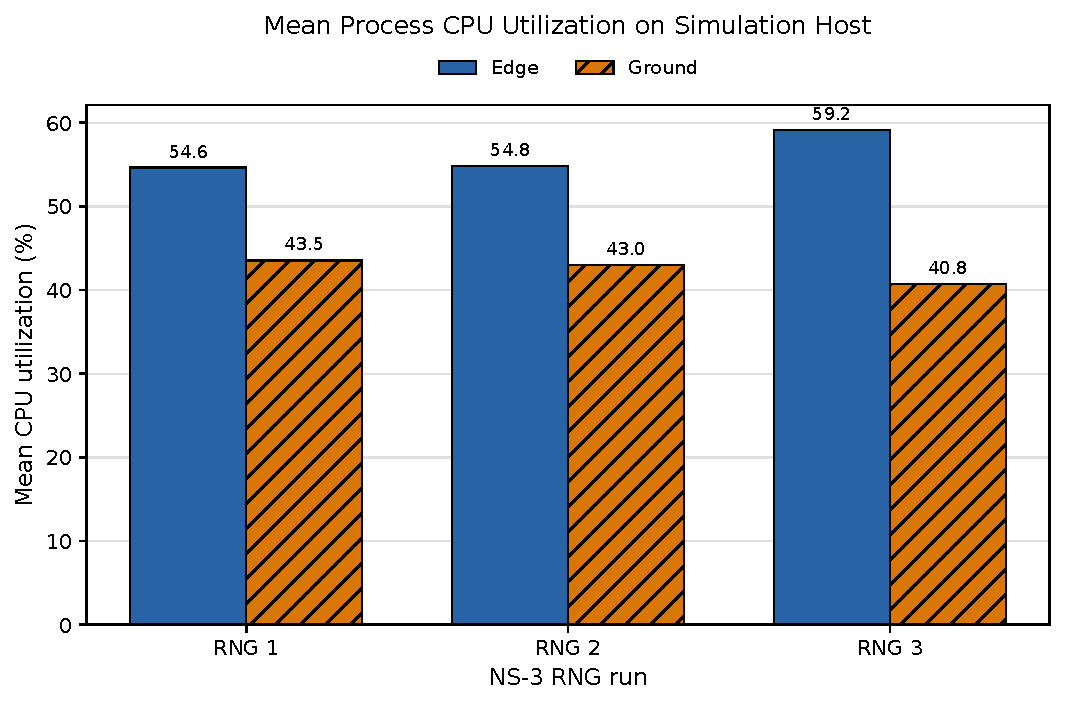
\includegraphics[width=0.78\textwidth]{images/application_layer_validation/mean_cpu_utilization_by_rng.pdf}%
    }{%
        \fbox{\parbox[c][0.28\textheight][c]{0.85\textwidth}{\centering Figure file not found.}}%
    }
    \caption{Mean monitored detector-plus-relay CPU utilisation on the simulation host.}
    \label{fig:mean-cpu-utilisation-by-rng}
\end{figure}

\subsection{Summary of Validation Results}
\label{subsec:testing-detection-summary}

\begin{table}[H]
    \centering
    \caption{Summary of the main application-layer validation results.}
    \label{tab:application-validation-summary}
    \begin{tabular}{|l|c|c|}
        \hline
        Metric & Edge/raw & Ground/JPEG q5 \\ \hline
        Processed-frame ratio & $1.0000 \pm 0.0000$ & $0.7667 \pm 0.0727$ \\ \hline
        Mean of run-level median latency & $182.41 \pm 19.22$ ms & $507.86 \pm 4.34$ ms \\ \hline
        Detection recall & 0.810651 & 0.171598 \\ \hline
        Detection F1-score & 0.843077 & 0.292929 \\ \hline
        Mean monitored CPU & $56.22 \pm 2.56\%$ & $42.44 \pm 1.47\%$ \\ \hline
        Mean monitored RSS & $952.32 \pm 5.11$ MB & $963.34 \pm 2.58$ MB \\ \hline
    \end{tabular}
\end{table}

Under the tested configuration, Edge produced result records for every officially published frame, while Ground had a lower processed-frame ratio. Edge also had lower run-level median latency. Raw images gave higher recall and F1-score than JPEG-quality-5 images. The monitored Edge processes used more mean CPU, while memory use was similar. The wider interpretation and limitations of these results are considered in the main Discussion and Limitations sections.
